%%%%%%%%%%%%%%%%%%%%%%%%%%%%%%%%%%%%%%%%%%%%%%%%%%%%%%%%%%%%%%%%%%%%%%%%%%%%%%%%%%%%%
\section{Conclusions}\label{sec:conclusions}
%%%%%%%%%%%%%%%%%%%%%%%%%%%%%%%%%%%%%%%%%%%%%%%%%%%%%%%%%%%%%%%%%%%%%%%%%%%%%%%%%%%%%

This dissertation, "Leveraging Multi-Messenger Astrophysics for Dark Matter Searches," advances our quest to understand dark matter. We used gamma-ray and neutrino observatories alongside advanced computational techniques. Our goal was to enhance the search for dark matter within the universe.

The Glory Duck project was a key part of this work. It involved a multi-instrument analysis using gamma-ray telescopes. These included Fermi-LAT, H.E.S.S., MAGIC, VERITAS, and HAWC. They focused on 20 dwarf spheroidal galaxies (dSphs). The aim was to detect dark matter annihilation signals. Although we found no significant deviations from the null hypothesis, we greatly improved search sensitivity. We set stringent upper limits on the annihilation cross-section for dark matter candidates. This effort represents a major advance, offering the most comprehensive constraints for WIMP dark matter search to date.

Our exploration of multithreading techniques in HAWC analyses showed the benefits of computational methods. By accelerating analysis time, we enhanced the efficiency of dark matter searches. This approach has set the stage for more ambitious studies. It highlights the importance of computational innovation in addressing astrophysical challenges.

Furthermore, our work with IceCube's North Sky Track Data has broken new ground. It aimed at detecting heavy dark matter annihilation. We used parallel programming and spline fitting to improve IceCube's sensitivity. This analysis is a step towards probing dark matter annihilation up to the PeV scale. It demonstrates a significant sensitivity improvement compared to previous efforts. The groundwork laid here is a strong foundation for future discoveries.

This dissertation highlights the potential of multi-messenger astrophysics and computational innovation in dark matter searches. Each analysis has contributed to our understanding and capabilities. Together, they showcase a progressive approach to astrophysical research. By integrating observations and using the latest computational techniques, we have expanded our capabilities. We have also charted a path for future dark matter searches.

Looking back, it's clear that our journey through the dark universe is far from complete. The methods developed and findings reported here significantly contribute to the astrophysical community. They set the stage for future multi-messenger observations and analyses. In this pursuit, the challenges we face and the questions we seek to answer drive us forward. They fuel the continuous evolution of our search for dark matter.

%%%%%%%%%%%%%%%%%%%%%%%%%%%%%%%%%%%%%%%%%%%%%%%%%%%%%%%%%%%%%%%%%%%%%%%%%%%%%%%%%%%%%
\section{Future Directions: Multi-Messenger Dark Matter Search}\label{sec:future}
%%%%%%%%%%%%%%%%%%%%%%%%%%%%%%%%%%%%%%%%%%%%%%%%%%%%%%%%%%%%%%%%%%%%%%%%%%%%%%%%%%%%%

\begin{figure}[h]
    \centering{
        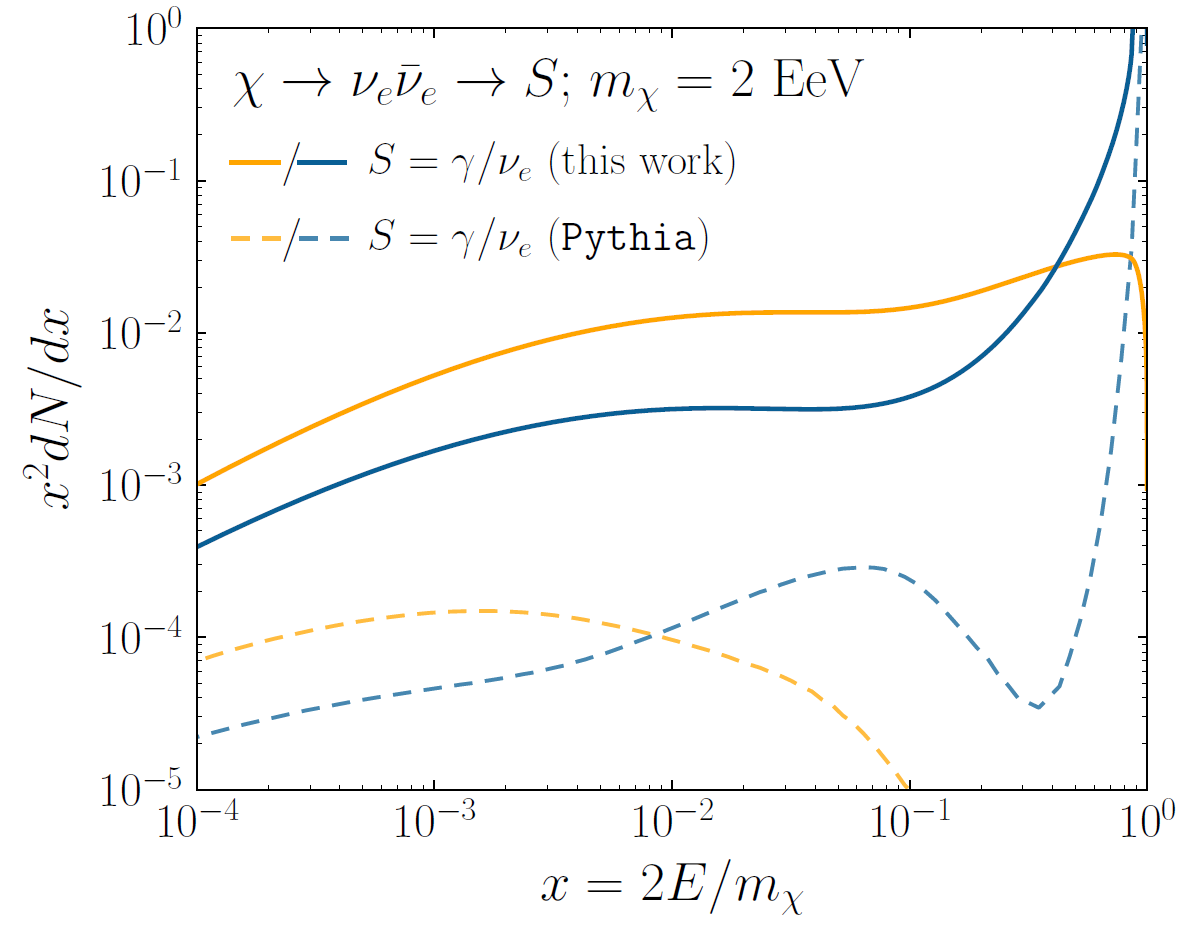
\includegraphics[scale=0.4]{figures/hdm_gamma_nu.png}
    }
    \caption{The prompt electron neutrino and photon spectrum resulting from the decay of a 2EeV DM particle to \parpar{\nu_e}, as currently being searched for at IceCube [5]. Solid curves represent the results of this work, and predict orders of magnitude more flux at certain energies than the dashed results of Pythia 8.2, one of the only existing methods to generate spectra at these masses. In both cases energy conservation is satisfied: there is a considerable contribution to a $\delta$-function at x = 1, associated with events where an initial W or Z was never emitted and thus no subsequent shower developed. Large disagreements are generically observed at these masses for electroweak dominated channels, while the agreement is better for colored initial SM states.}
    \label{fig:nu_and_gam}
\end{figure}

As I have shown previously in \cref{sec:glory_duck} and \cref{sec:multithread}, we can build a fast and robust analysis that shares tools with the field.
The hope being that IceCube can eventually combine data with gamma-ray observatories.
\tmpfig{nuetrino and bb plot with nu Sensitivities}